\documentclass[border=5mm]{standalone}
\usepackage{tikz}
\usetikzlibrary{calc, intersections}

\begin{document}
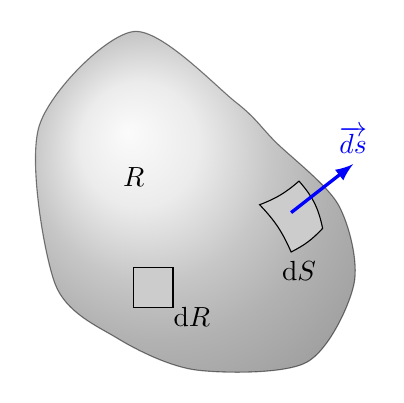
\begin{tikzpicture}

\shadedraw[ball color=gray!40,opacity=0.5] plot[smooth cycle] coordinates {(-2,1) (-0.8,2.2) (0.5,1.3) (1,0.8) (1.8,0)
(2,-1) (1.4,-2) (0,-2.1) (-1,-1.7) (-1.8,-1)};
\draw[fill=gray!40] (0.8,0) to[bend right=10] (1.3,0.3) to[bend left=15] (1.6,-0.3)
to[bend left=10] (1.2,-0.6) to[bend right=10] cycle;
\draw[blue,very thick,-latex] (1.2,-0.1) -- ++(38:1) node[above] {$\overrightarrow{ds}$};
\node[anchor=north] at (1.3,-0.6) {d$S$}; 
\node[anchor=north] at (-0.8,0.6) {$R$}; 
\draw[fill=gray!40] (-0.8,-0.8) rectangle (-0.3,-1.3) node[below right=0pt,
inner sep=0pt]{d$R$};

\end{tikzpicture}
\end{document}

